\documentclass[acmsmall]{acmart}\settopmatter{printfolios=true,printccs=false,printacmref=false}

\usepackage{booktabs} % For formal tables

\usepackage{blindtext}

% TOG prefers author-name bib system with square brackets
\citestyle{acmauthoryear}
%\setcitestyle{square}

\usepackage{listings}
\usepackage{xcolor}

\usepackage{tikz}
\tikzset{main node/.style={circle,draw,minimum size=1cm,inner sep=0pt},
            }

\lstdefinelanguage{scala}{
	morekeywords={abstract,case,catch,class,def,%
	do,else,extends,false,final,finally,%
	for,if,implicit,import,match,mixin,%
	new,null,object,override,package,%
	private,protected,requires,return,sealed,%
	super,this,throw,trait,true,try,%
	type,val,var,while,with,yield},
	otherkeywords={=>,<-,<\%,<:,>:,\#,@},
	sensitive=true,
	morecomment=[l]{//},
	morecomment=[n]{/*}{*/},
	morestring=[b]",
	morestring=[b]',
	morestring=[b]"""
}
	
\definecolor{dkgreen}{rgb}{0,0.6,0}
\definecolor{gray}{rgb}{0.5,0.5,0.5}
\definecolor{mauve}{rgb}{0.58,0,0.82}

% \lstdefinestyle{myScalastyle}{
% 	frame=tb,
% 	language=scala,
% 	aboveskip=3mm,
% 	belowskip=3mm,
% 	showstringspaces=false,
% 	columns=flexible,
% 	basicstyle={\small\ttfamily},
% 	numbers=left,
% 	numberstyle=\tiny\color{gray},
% 	keywordstyle=\color{blue},
% 	commentstyle=\color{dkgreen},
% 	stringstyle=\color{mauve},
% 	frame=single,
% 	breaklines=true,
% 	breakatwhitespace=true,
% 	tabsize=2,
% }
\lstset{
	basicstyle=\ttfamily,
	captionpos=b,
	%breaklines=true,
	%showstringspaces=false,
	%tabsize=2,
	%frame=lines,
	%numbers=left,
	%numberstyle=\tiny,
	%xleftmargin=2em,
	%framexleftmargin=2em
}

\usepackage[ruled]{algorithm2e} % For algorithms
\renewcommand{\algorithmcfname}{ALGORITHM}
\SetAlFnt{\small}
\SetAlCapFnt{\small}
\SetAlCapNameFnt{\small}
\SetAlCapHSkip{0pt}
\IncMargin{-\parindent}

\bibliographystyle{ACM-Reference-Format}

% Metadata Information
\acmJournal{CSUR}
%\acmVolume{1}
%\acmNumber{CONF} % CONF = POPL or ICFP or OOPSLA
\acmArticle{1}
\acmYear{2018}
\acmMonth{4}

% Copyright
\setcopyright{none}
%\setcopyright{acmcopyright}
%\setcopyright{acmlicensed}
%\setcopyright{rightsretained}
%\setcopyright{usgov}
%\setcopyright{usgovmixed}
%\setcopyright{cagov}
%\setcopyright{cagovmixed}

% DOI
%\acmDOI{0000001.0000001_2}

% Paper history
\received{April 2018}
%\received{March 2009}
%\received[final version]{June 2009}
%\received[accepted]{July 2009}
\usepackage{layouts}

\usepackage[belowskip=-15pt,aboveskip=0pt]{caption}

% Document starts
\begin{document}

%\setlength{\textfloatsep}{\baselineskip plus 0.2\baselineskip minus 0.2\baselineskip}
% Title portion
\title{A survey on Deprecating the Observer Pattern}

\author{Joel Bartelheimer}
\affiliation{%
\institution{Technische Hochschule Mittelhessen--University of Applied Sciences}
\city{Giessen}
\state{Hessen}
\postcode{35390}
\country{Germany}}
\email{joel.bartelheimer@mni.thm.de}


\renewcommand\shortauthors{Bartelheimer, J. }

\begin{abstract}
	\blindtext
\end{abstract}


%
% The code below should be generated by the tool at
% http://dl.acm.org/ccs.cfm
% Please copy and paste the code instead of the example below.
%
\begin{CCSXML}
	<ccs2012>
	<concept>
	<concept_id>10011007.10011074.10011075.10011077</concept_id>
	<concept_desc>Software and its engineering~Software design engineering</concept_desc>
	<concept_significance>500</concept_significance>
	</concept>
	<concept>
	<concept_id>10011007.10011074.10011075.10011078</concept_id>
	<concept_desc>Software and its engineering~Software design tradeoffs</concept_desc>
	<concept_significance>300</concept_significance>
	</concept>
	<concept>
	<concept_id>10011007.10011074.10011075.10011079</concept_id>
	<concept_desc>Software and its engineering~Software implementation planning</concept_desc>
	<concept_significance>300</concept_significance>
	</concept>
	</ccs2012>
\end{CCSXML}

\ccsdesc[500]{Software and its engineering~Software design engineering}
\ccsdesc[300]{Software and its engineering~Software design tradeoffs}
\ccsdesc[300]{Software and its engineering~Software implementation planning}
%
% End generated code
%
\keywords{design patter, observer pattern, event handling, data-flow language, reactive programming, user interface programming, scala}
\maketitle

%input

\section{Introduction}
	%batch programs -> reactive application
	%hard to programm
	%we need better programmin abstractions for reactive programming
	%first approache is the observer pattern
	%researcher addressed the problems
	%new languages features and abstractions for the new problems
	

	In contrast to traditional batch mode programs modern applications are reactive and event driven. 
	examples like the GUI 
	reactive is hard and errorprone, dealing with continuous event occurrence and user input requires a considerable amount of engineering.
	
	quote an Adobe presentation from 2007~\cite{parent2006possible} on current production systems:
	\begin{itemize}
		\item 1/3 of the code in Adobe’s desktop applications is devoted to event handling logic	
		\item 1/2 of the bugs reported during a product cycle exist in this code
	\end{itemize}


	
	A programming paradigm well suited for these event-driven and interative applications is reactive programming
	reactive programming gained popularity

	early approach in reactive programming is the use of the observer Pattern
	
	\subsection{UI Event handling}



	in the paper ``Deprecating the Observer Pattern'' the authors criticize the use of the observer pattern for reactive programs,
	the title already is a hard claim by itself.



\section{Observer Pattern}
	The observer pattern was originally published in \cite{Gamma:1995}. 
	It is one of the behavior patterns by the Gang of Four. 
	The intent of the observer pattern is a one-to-many dependency with an automatic change propagation.
	When the state of an object (one) changes, all it dependents objects (many) are notified automatically.

	\begin{figure}[H]
		\includegraphics{img/observer.jpg}
		\caption{Structure of the observer pattern~\cite{Gamma:1995}}
		\label{fig:observer}
	\end{figure}

	The observer pattern consists of four components, their relations and methods are shown in figure~\ref{fig:observer}.

	\begin{description}
		\item[Subject] Provides an interface for installing (\textit{attach}) and uninstall (\textit{detach}) observers. 
		Moreover, the subject knows its observers and the number of observers is not limited.
		\item[Observer] The \textit{update} method is the observers updating interface for receiving changes in a subject.
		\item[ConcreteSubject] Stores the state, where the observers are interested in and also initiates the notification when the state changes.
		\item[ConcreteObserver] Implements an updating interface to keep its stored state of the subject consistent. 
	\end{description}

	In the original source various slightly different implementation are discussed. 
	One of them deals with the update and how the observers receive the changed data. 
	Often the subject passes additional information as an argument to the \textit{update} method, e.g. a changed mouse position. 
	To avoid observer-specific update protocols, two extreme cases -- \textit{push model} and \textit{pull model}-- are described.
	With the \textit{push model}, the subject sends detailed information to the observers about the changed state, even if the observers are not interested. 
	On the opposite, nothing is sent by the subject only the change notification, the observers have to ask for the information afterward~\cite{Gamma:1995}.
	Usually implementations, e.g. the Java \textit{Observable} implementation~\cite{oracleObservable}, support both models.

	%why the observer for event handling
	For event handling, the subject receives the actual event, e.g. a mouse click, and notifies all its observers.
	And because of the Observer pattern, the event consumers are decouple from the source of the event. 
	Therefore, typical use cases for the observer pattern are graphical user interfaces.
	Also many GUI related frameworks closely follow the observer pattern, e.g. Smalltalk's Model/View/Controller or Java Swing~\cite{Gamma:1995,Maier:2010}.
	%but.. 
	\subsection{Violations of software engineering principles}
		In \cite{Maier:2012} it is shown by means of code exmples that the observer pattern violates a set of software engineering principles,
		particularly for the use of event handling in interactive GUI applications.
		The violated principles are:
		\begin{description}
			\item[Side-effects]
			Often several observers are used to implement a single Operation,
			e.g. a \lstinline|onClick| and a \lstinline|onRelease| observer are necessary to implement a drag and drop operation.
			Therefore, the observer patterns promote side-effects and already on the API level.
			
			\item[Encapsulation]
			In many cases multiple observers are used to simulate a state machine. 
			The state, e.g. a dragged object, is stored in a variables within a shared scope.
			As this broader scope of these shared variables escapes the scope of the observers, the observer pattern violates the encapsulation principle.
			
			\item[Composability]
			Observers are registered during runtime on various installation points.
			Even if multiple observers deal with a single concern, like a drag and drop operation, it is not possible to, e.g. easily add or remove drag behavior.
			
			\item[Resource management]
			The installation and uninstallation of a observer has to be managed explicitly.
			The mouse movement for instance, should only be observed during a drag operation, due to performane. 
			Therefor the client is in charge to manage the observers life-time.
			
			\item[Separation of concerns]
			Usually a observer deals with more than on concern. For instance, recalculating and refreshing the state and also drawing the new state changes.
			That a single observer deals with multiple concerns is not recommendable, the concerns shall be seperated.

			\item[Data consistency]
			The separation of concerns can be archived by limiting the concerns a observer deals with to one and then the observer itself publishes events on change.
			Each concern can then observe its dependent concerns.
			But unfortunately, there is no guarantee for data consistency when a observer listens to multiple changes. 
			% B A
			% |/|
			% C |
			% |/
			% D
			\begin{figure}[H]
				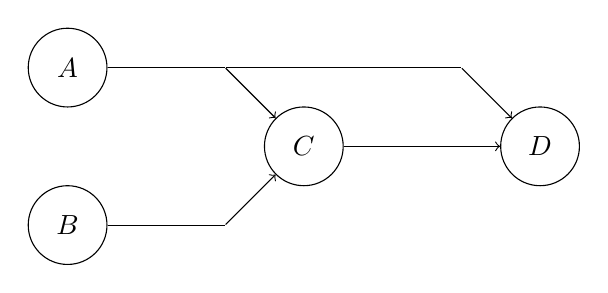
\begin{tikzpicture}
					\begin{scope}[xshift=8cm]
						\node[main node] (A) at (0,0) {$A$};
						\node[main node] (B) at (0,-2) {$B$};
						\node[inner sep=0,minimum size=0] (K1) at (2,0) {};
						\node[inner sep=0,minimum size=0] (K3) at (2,-2) {};
						\node[main node] (C) at (3,-1) {$C$};
						\node[inner sep=0,minimum size=0] (K2) at (5,0) {};
						\node[main node] (D) at (6,-1) {$D$};
						
						\draw[-] (A) to (K1);
						\draw[->] (K1) to (C);
						\draw[-] (K1) to (K2);
						\draw[->] (K2) to (D);
						\draw[-] (B) to (K3);
						\draw[->] (K3) to (C);
						\draw[->] (C) to (D);
					\end{scope}
				\end{tikzpicture}
				\caption{Dependency graph}
				\label{fig:glitchgraph}
			\end{figure}
			Figure~\ref{fig:glitchgraph} shows a dependency graph where \textit{C} observes changes from \textit{A} and \textit{B} and \textit{D} observes the resulting \textit{C} and also \textit{A}.
			When \textit{A} emits a change event, \textit{D} can not determine if \textit{C} has already consumed the change or not. 
			The short moment, where \textit{C} has not consumed the change event, is called a \textit{glitch}.
			\item[Uniformity]
			Every subject provides its own installation point for observers, which decreases code uniformity.
			\item[Abstraction]
			The use of heavyweight interfaces is promoted by the observer pattern. 
			Often, much more methods than just one to install a specific observer is provided. 
			Therefore, it is not possible to abstract over a precise event source, e.g. when we want to use pointer events instead of mouse events.
			\item[Semantic distance]
			The observer pattern reverses the control flow -- the subject invokes the \lstinline|update()| method of the observer -- which results in more boilerplate code and makes the code harder to understand.
		\end{description}
		
		Nearly half of the violations are caused by dealing with multiple observers.
		But exactly the feature of chaining and composing multiple observers together is not mentioned in the original source~\cite{Gamma:1995}.

\section{Reactive programming}
	Reactive programming is a paradigm which provides dedicated programming abstraction for interactive and event-driven applications.
	As mentioned in the introduction, designing, implementing and maintaining reactive application is not an easy task. 
	The code of a program is triggered asynchronously by the occurrence of events.
	For this reason, developers struggle to understand the control flow of an application.
	The approach of reactive programming is, to express these complex reactive behaviors in an intuitive and declarative way.
	The following are the core principles of reactive programming~\cite{Salvaneschi:2015,Salvaneschi:2017}:

	\begin{description}
		\item[Declarativeness] Instead of computational steps, to derive a new component state based on a prior state,
		programmers address \textit{how} components functionally depend on each other.
		\item[Abstraction over change propagation] Change Propagation of dependent values is done implicit by the underlying execution model instead of manually by the developer.
		\item[Composability] Reactive computations can be composed to more complex computations by using provided abstractions (e.g., combinators/operator for event streams).
		\item[Favoring data flow over control flow] Normally the excecution of an application follows the control flow. 
		In reactive programming the computation is driven by events and data and how they flow through the system.
	\end{description}

	To explain these principle a short example is given:

	\begin{lstlisting}
		var1 = 1
		var2 = 2
		var3 = var1 + var2
	\end{lstlisting}

	In conventional sequential imperative programming, 
	the variavle \lstinline|var3| has the initial value of the sum of \lstinline|var1| and \lstinline|var2|, which is 3.
	And when afterwards a new value is assigned to variable \lstinline|var1| or \lstinline|var2| the value of \lstinline|var3| remains.
	Only with an explicit assignment, the value of varialbe \lstinline|var3| can be changed. In contrast to reactive programming, 
	where variable \lstinline|var3| is always up-to-date. Whenever the value of \lstinline|var1| or \lstinline|var2| changes, 
	the reactive execution model recomputes the new value for \lstinline|var3|~\cite{Bainomugisha:2013}.
	
	\subsection{Basic abstractions}
	In reactive programming languages and frameworks two distinguished features or abstractions are used, signals and events.
	time-varying values(signals or behaviors)
	event streams
	%automatic tracking of dependencies
	%automated change propagation
	\cite{Salvaneschi:2015}

	\subsection{Functional reactive programming}
		Reactive programming has its origin in Functional reactive programming, a variation for strictly functional languages. 
		first in functional languages by~\cite{Elliott}
		focus on modeling time in pure functional languages
		signals behaviour~\cite{Bainomugisha:2013}
	

\section{Scala.React}

	\subsection{First class events}

	\subsection{Reactor}

	\subsection{Embedded dataflow langugage}

	\subsection{Glitch avoidance}

\section{Evolution of reactive programming frameworks}
	
	different types of frameworks, research driven or by practitioners in the software community
	research driven implement all principles and abstractions
	practitioners focus on a specific fields like gu

	with lambda-expressions and stream java added data-flow elements to the language for more declarative programming
	added in java 8 and already extended in java 9

	most 

	\subsection{Reactive databinding}

		Font-end frameworks inspired by the Flapjax reactive language~\cite{Meyerovich:2009}

		Metor example: ~\cite{hochhaus2016meteor}

		based on fl

	\subsection{Reactive streams}

\section{Conclusion}


%as seen, reactive frameworks evolved and 
reactive programming gained popularity~\cite{reactiveManifesto2014}, also spread to other fields like cloud computing and big data \cite{Salvaneschi:2015}

glitch avoidance not always important. only in singlethreaded push based enviroments like gui-threads

%appendix: 
%javafx not glitch free stack overflow: https://stackoverflow.com/questions/25139257/terminology-what-is-a-glitch-in-functional-reactive-programming-rx

% Bibliography
\bibliography{sources}

\end{document}
